\documentclass[a4paper, 12pt]{article}
\usepackage{a4wide}
\usepackage{textcomp}
\usepackage{listings}
\usepackage{color}

\usepackage{graphicx}
\graphicspath{ {./images/} }

\usepackage[backend=biber,style=numeric]{biblatex}
\addbibresource{bibliography.bib}

\definecolor{dkgreen}{rgb}{0,0.6,0}
\definecolor{gray}{rgb}{0.5,0.5,0.5}
\definecolor{mauve}{rgb}{0.58,0,0.82}

\lstset{frame=tb,
  language=Java,
  aboveskip=3mm,
  belowskip=3mm,
  showstringspaces=false,
  columns=flexible,
  basicstyle={\small\ttfamily},
  numbers=none,
  numberstyle=\tiny\color{gray},
  keywordstyle=\color{blue},
  commentstyle=\color{dkgreen},
  stringstyle=\color{mauve},
  breaklines=true,
  breakatwhitespace=true,
  tabsize=3
}

\begin{document}

    \title{A Graphical Programming Language Editor}
    \author{Candidate No. 198719}
    \date{November 3, 2020}
    \clearpage\maketitle
    \thispagestyle{empty}

    \newpage\clearpage\thispagestyle{empty}
    \tableofcontents
    \newpage
    \setcounter{page}{1}

    \section{Introduction}
    Graphical programming can be a fantastic and intuitive way to introduce new programmers to
    the scene. When programmers ask others for assistance, those helping typically do so in a visual 
    style, using whiteboards, drawing flowcharts, with boxes and arrows indicating the flow 
    of the program. Why can't we make programs in the same style if we find it so helpful to read? 
    The concept behind graphical programming is specifying the elements of the program graphically 
    rather than textually~\cite{dehouck2015maturity}.

    Popular examples of graphical programming include Scratch, as well as a personal favourite that 
    I used during my GCSE Computing education, App Inventor!
    What's clever about Scratch is its simplicity due to the block-based visual programming, aimed 
    towards younger children to help them get into coding!

    \begin{figure}[h]
        \centering
        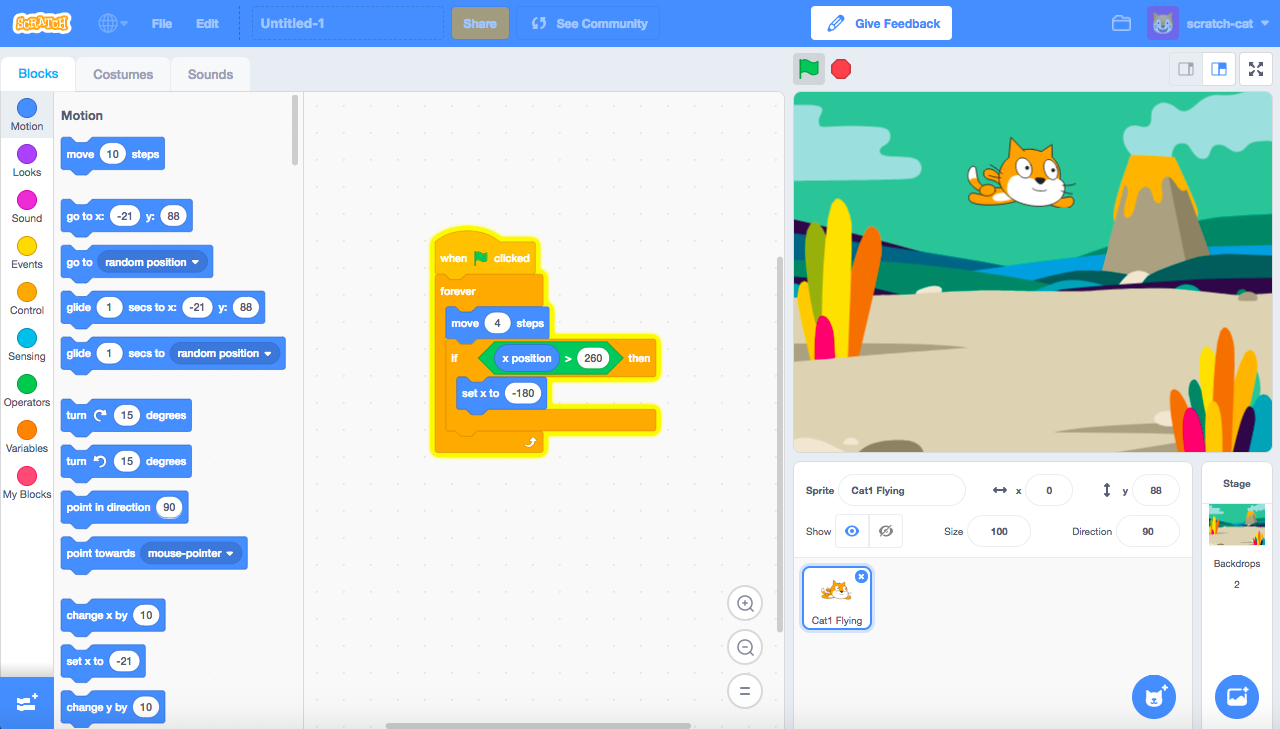
\includegraphics[width=160mm]{scratch_image}
        \caption{Scratch's visual scripting over a white canvas~\cite{thescratchteam}.}
    \end{figure}

    \clearpage
    MIT App Inventor is one of my personal favourites after experiencing it myself during GCSEs, 
    having to building an on-campus application for a University! It uses a graphical user 
    interface, similar to Scratch, as well as providing the blocks that you can use, visible on 
    the left hand side.

    \begin{figure}[h]
        \centering
        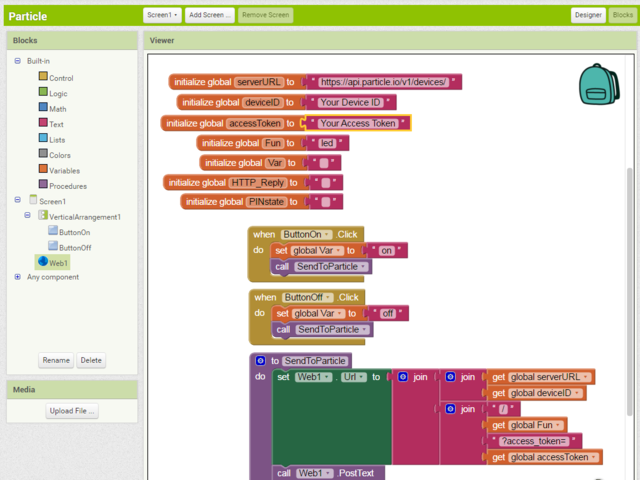
\includegraphics[width=150mm]{app_inventor}
        \caption{MIT App Inventor graphical programming~\cite{adafruit}.}
    \end{figure}

    Both what Scratch and App Inventor do superbly is colour code their blocks to identify 
    exactly what they are representing. There are colour coded blocks for variables, events 
    and controls, and so on! For instance in App Inventor, variables are coloured in Orange 
    blocks, and procedures and show in a big purple block, encapsulating all the blocks like 
    a function.

        \subsection{Aims}


        \subsection{Objectives}
    
        Needs of intended users. \\
        Brief description of the problem area. \\
        Motivation \\
        Project relevance. \\
        What will you do? \\ 
        How will you do it? \\ 
        Why will you do it? \\

        \subsection{Problem Area}
            The main challenge of implementing an interface to be able to program on is the required 
            time and skill set. This project may never be fully complete as more work can always be 
            done to improve the functionality of the interface, or making the interface more user-friendly.

            The project can be broken down into key areas that require focusing on:
        
            \begin{itemize}
                \item Graphical Design - modelling, interface, simplicity, GUI.
                \item Functionality - programming.
            \end{itemize}

            I have limited GUI design in Java from my 2nd year module, Further Programming, therefore this 
            process can be said to take up a large amount of time. Careful consideration is needed to 
            not overspend my time on the GUI design process, and rather get the functionality of said 
            interface to work.

            Functionality requires programming to be clean and efficient, so not to go back over the code 
            and forget what was written. Code must be documented and commented along the way to make sure 
            anyone who reads the code, including myself in the future, is able to understand what was 
            written and why it was decided.

            \subsection{Expected Outcomes}
            The expected outcomes of this project are a fully working, funtional graphical programming 
            language interface. The user should use the tool independent from the backend Java textual 
            code, and be able to perform the certain tasks:

            \begin{itemize}
                \item loops - create and work with basic for \& while loops.
                \item data structures - create and interact with data structures such as lists.
            \end{itemize}

    \section{Professional and Ethical Considerations}
        Discuss the ethical issues your prject is likely to deal with: \\
        - awareness of technological procedures and standards. \\
        - understanding and complying with legisaltion. \\
        If need humans, include plan and timetable for obtaining ethical approval.

    \section{Related Work}
        Scratch and App Inventor - I used app inventor for my GCSE assignment, making an application for a university campus.

        Do some background research. \\
        What has already been done in this field? \\
        How is your approach different and better than others? \\
        What is the novelty of your project, compared to others? \\
        What is your contribution to the field? \\
        Do not re-invent the wheel! \\

    \clearpage
    \section{Requirements Analysis}
        In this section, I have taken into careful consideration the aims and objectives for this
        project. Below you will find a compiled list of software requirements, split into two
        categories: \textbf{mandatory} requirements, the fundamental requirements that is needed
        for the project to work, and \textbf{desirable} requirements, optional further requirements
        that can be met to provide further quality of life experiences for the user.

        \subsection{Mandatory Requirements}

            \begin{table}[h]
                \begin{tabular}{|l|l|}
                    \hline
                    \multicolumn{2}{|c|}{\textbf{Mandatory Requirements}}                                                                                                                                                                                                            \\ \hline
                    \textbf{Requirement}                                                                                                     & \textbf{Specification}                                                                                                                \\ \hline
                    \begin{tabular}[c]{@{}l@{}}1. Application will work on any java-run\\ environment.\end{tabular}                          & \begin{tabular}[c]{@{}l@{}}Whether the user is on a Windows, Mac OSX\\ or Linux system, the application will work.\end{tabular}       \\ \hline
                    \begin{tabular}[c]{@{}l@{}}2. The interface shall accept user input\\ via keyboard and mouse.\end{tabular}               & \begin{tabular}[c]{@{}l@{}}User will be able to use keyboard and mouse\\ to create and interact with the canvas.\end{tabular}         \\ \hline
                    3. The program shall run until is it killed.                                                                             & \begin{tabular}[c]{@{}l@{}}The process will not stop running until either\\ it is killed via user or forced shutdown.\end{tabular}    \\ \hline
                    \begin{tabular}[c]{@{}l@{}}4. The program will output any errors,\\ if any.\end{tabular}                                 & \begin{tabular}[c]{@{}l@{}}If there are any run-time errors, the terminal\\ will output those for the user to see.\end{tabular}       \\ \hline
                    \begin{tabular}[c]{@{}l@{}}5. The user shall be able to use functional\\ loops such as for and while loops.\end{tabular} & \begin{tabular}[c]{@{}l@{}}The user will have the ability to interact with\\ loops in the interface.\end{tabular}                     \\ \hline
                    \begin{tabular}[c]{@{}l@{}}6. The user shall be able to create\\ variables.\end{tabular}                                 & \begin{tabular}[c]{@{}l@{}}The user will be able to create and interact\\ with variables.\end{tabular}                                \\ \hline
                    \begin{tabular}[c]{@{}l@{}}7. The user shall be able to create\\ functions or procedures.\end{tabular}                   & \begin{tabular}[c]{@{}l@{}}Users will have the ability to create functions\\ /methods that perform a variety of tasks.\end{tabular}   \\ \hline
                    \begin{tabular}[c]{@{}l@{}}8. The user will be able to create data\\ structures.\end{tabular}                            & \begin{tabular}[c]{@{}l@{}}Data structres such as lists will be available\\ for the user to implement and interact with.\end{tabular} \\ \hline
                \end{tabular}
            \end{table}


        The main

        Does your project meet the needs of a target group of users? \\
        What are the needs of these target users? \\
        How would an ideal system meet their needs? \\
        To what extent does your solution contribute to this? \\
        What do you expect to achieve within the given time? \\
        What will you definitely not achieve? \\
        You should stick to this analysis till the end of your project!

    \clearpage
    \section{Project Plan}
        Describe what you have already done. \\
        Schedule what you still want to do. \\
        How are your tasks interdependent? \\
        Writing the draft report should be one of your main tasks.

    \section{Interim Log}
        Log of the meetings with your supervisor. \\
        Should cover discussions of every important project stage. \\
        Record the prupose and the outcome of every meetings. \\
        Note how these meetings helped you follow your plan. \\
        Include this log as an appendix to your report.
    
    \section{Appendices}
        \subsection{Project Proposal}

    \printbibliography
\end{document}